\documentclass[a4paper,12pt]{article}
\usepackage{latexsym}
\usepackage{rotate}
%\usepackage{../texstuff/chicago}

\usepackage{graphics}

%\bibliographystyle{../texstuff/chicago}
%\renewcommand{\labelenumi}{(\roman{enumi})}
\newcommand{\eps}{\epsilon}
\newcommand{\var}{{\rm var}}
\newcommand{\cov}{{\rm cov}}
\newcommand{\nid}{{\rm NID}}
\newcommand{\diag}{{\rm diag}}
\newcommand{\E}{{\mathrm E}}
\newcommand{\R}{{\mathrm R}}
\newcommand{\U}{{\mathrm U}}
\newcommand{\Ex}{{\cal E}}
\newcommand{\cor}{\mathrm{cor}}
\newcommand{\tr}{\mathrm{tr}}
\newcommand{\e}{\mathrm{e}}
\newcommand{\de}{\mathrm{d}}
\newcommand{\p}{\mathrm{P}}
\newcommand{\Ln}{\mathrm{Ln}}
\newcommand{\ra}{\varrho}

\newcommand{\eref}[1]{(\ref{#1})}
\newcommand{\fref}[1]{Figure \ref{#1}}

\begin{document}

\title{Structured copula modelling of insurance liabilities}
\author{Piet de Jong
\\\\ \small Department of Actuarial Studies, \\ \small Macquarie
University, NSW 2109, Australia. \\ \small Email:
piet.dejong@mq.edu.au}

\date{}
\maketitle

\begin{abstract}
This article employs copulas to model total claims losses arising from different lines of insurance.   There are two contributions.   First a flexible method is developed to generate copulas.   Second total losses are considered given the marginal distributions are Weibull.
\end{abstract}

\paragraph{Keywords:}Copulas

\section{Introduction}

This article develops and discusses a practical, structural way of generating copulas.   By structural we mean the copula is generated from a generating mechanism typical of statistical modeling.   This contrasts with the usual way of specifying copulas directly via functional forms as discussed for example in \citeN{joe1997mma} or \citeN{nelsen2006ic}.

\fref{fig1} displays  simulations from a copula constructed using  the proposed copula generating method. Each  panel in \fref{fig1} is generated by firstly simulating for $t=1,\ldots, N$ from the bivariate distribution
\begin{equation}\label{chi1}
s_{1t}=\alpha_t\ , \qquad s_{2t}=\alpha_t+\ln(\rho)\eps_t\ , \qquad \alpha_t\sim\chi_1^2\ ,\qquad \eps_t\sim N(0,1)\ .
\end{equation}
where $\chi^2_1$ denotes the chi--squared with 1 degree of freedom, and $0\le\rho\le 1$. Given simulated values $s_{1t}$ and $s_{2t}$, the corresponding percentiles $G(s_t)\equiv \{G_1(s_{1t},G_2(s_{2t})\}'$ are calculated where the $G_i$ denote marginal distributions.   Since $G$ is not specified directly, the percentiles are estimated by the percentile ranks $\check s_{1t}$ and $\check s_{2t}$, that is their ranks in the simulated sample divided by the sampling effort $N$.

\begin{figure}[htb]
\centering
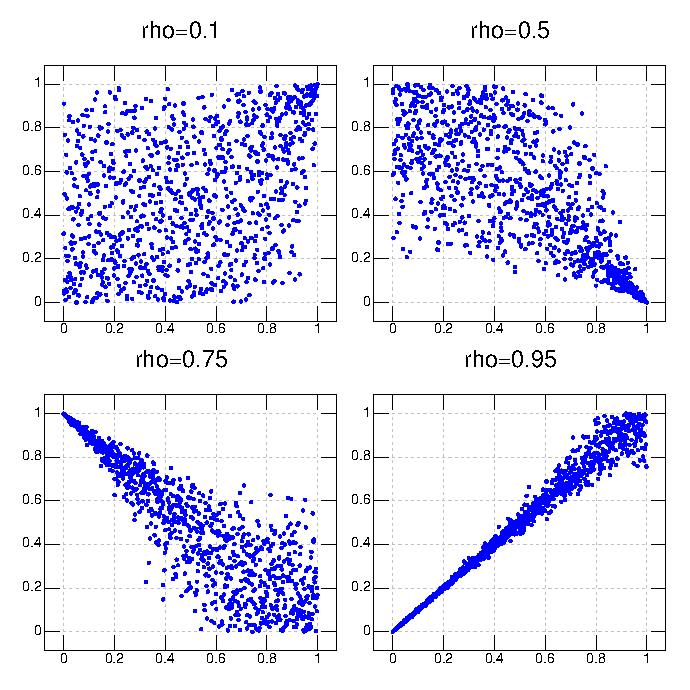
\includegraphics{fig1.eps}
\caption{Simulated percentile ranks $(\check s_{it},\check s_{2t})$ from model (\ref{chi1}).} \label{fig1}
\end{figure}

In \fref{fig1}, if $\rho\approx 0$ then $\ln(\rho)$ is very negative and $s_{1t}$ and $s_{2t}$ are virtually unrelated since $s_{2t}$ is dominated by $\ln(\rho)\eps_t$.  If $\rho\approx 1$ then $\ln(\rho)\approx 0$ and $s_{1t}$ and $s_{2t}$ are highly dependent.  The panels in \fref{fig1} suggest increasing upper tail dependence in that the conditional probability $P(\check s_{2t}> u|\check s_{1t}>u)$ increases as $u\rightarrow 1$.

The chi--squared specification for $\alpha_t$ can be changed to other extreme value or heavy tailed distributions. For example the log--normal is an alternative.  \fref{fig2} illustrates the copula when $\alpha_t\sim t_1$, in (\ref{chi1}), a ``t"  random variable with 1 degree of freedom.  In this case tail dependence appears to increases in both tails. Thus when $\alpha_t$ is near zero, the effect of $\eps_t$ is to mask the dependence while if $|\alpha_t|$ is large the dependence increases: the perturbing effect of $\eps_t$ in these cases is negligible.

\begin{figure}[htb]
\centering
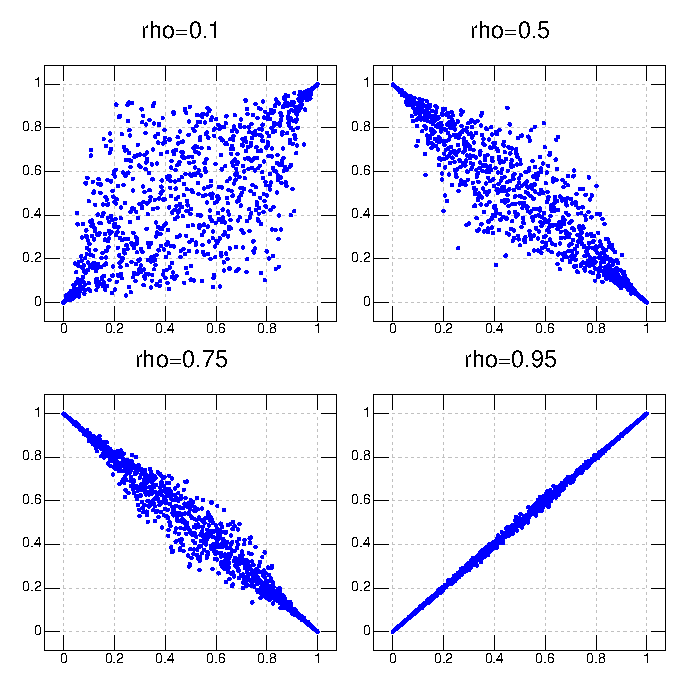
\includegraphics{fig2.eps}
\caption{Simulated percentile ranks from model (\ref{chi1}) if $\alpha_t\sim t_1$\ .}\label{fig2}
\end{figure}

The copula generating method \eref{chi1} generalizes the Gaussian copula \cite{mcneil2005qrm}.   If $\alpha_t\sim N(0,1)$ then $s_{1t}$ and $s_{2t}$ are jointly normal with correlation
$
    1/\sqrt{1+(\ln\rho)^2}
$.
Thus  in this case the relationship between the percentiles is induced with a Gaussian copula.  The Gaussian copula  combined with Gaussian marginal distributions for the actual observed variables yields the usual factor model often employed in the study of correlated data \cite{dnlawley1971fas}.


\section{The general form of the model}

Setup \eref{chi1} can be written in the vector form
    \begin{equation}\label{mat2}
        \left(
    \begin{array}{c}
      s_{1t} \\
      s_{2t} \\
    \end{array}
  \right)=
\left(
  \begin{array}{c}
    1 \\
    1 \\
  \end{array}
\right)
\alpha_t + \left(
              \begin{array}{cc}
                0 & 0 \\
                0 & \ln\rho \\
              \end{array}
            \right)\eps_t\ ,
    \end{equation}
This suggests the generalization
 \begin{equation}\label{mcop}
     \left(
    \begin{array}{c}
      s_{1t} \\
      s_{2t} \\
      \vdots\\
      s_{pt}
    \end{array}
  \right)=
\left(
  \begin{array}{c}
    1 \\
    1 \\
    \vdots \\
    1
  \end{array}
\right)
\alpha_t + \left(
              \begin{array}{cccc}
                \ln \rho_1 & 0 & \cdots & 0 \\
                0 & \ln\rho_2 & \cdots & 0 \\
                \vdots & \vdots & \ddots & \vdots \\
                0 & 0 & \cdots & \ln \rho_p \\
              \end{array}
            \right)\eps_t\ ,\qquad \eps_t\sim N(0,I)\ ,
  \end{equation}
  where the vector random variable $\alpha_t$ has an appropriate long tail distribution, and $\rho_1=1$.

  The general form of the proposed model is
\begin{equation}\label{gfac}
   y_t=F^-(\check s_t)\ , \qquad  s_t = Z\alpha_t + \psi\cdot\eps_t\ , \qquad \eps_t\sim N(0,I)\ .
\end{equation}
Here $\check s_t$ is the vector of percentiles of each component of $s_t$.  Further $\alpha_t$ is a vector of independent random variables with a heavy tailed distribution.  Further $\psi$ is a vector with entries $\ln(\rho_j)$ where $\rho_1=1$, the $\cdot$ notation indicates componentwise product, and $Z$ is a matrix of factor loadings.  The vector function $G$ is the vector of marginal distributions determined the joint distribution of $s_t$.  In particular component $i$ of $G(s_t)$ is $G_i(s_{it})$ where $G_i$ is the marginal distribution of $s_{it}$, component $i$ of $s_t$.  The vector of functions $F$ is similarly defined in terms of the marginal distributions of $y_t$, and $F^-$ denotes the vector of inverse mapping.

Analogous to state space models in time series, $\alpha_t$ is the ``state" vector, driving the tail dependence or tail correlation in the system.  Thinking of a one--dimensional state, when $\alpha_t$ is large

The marginal distributions in $G$ are easy to describe and simulate from but functional forms for the specific cases of interest are usually not available.   For example if $\alpha_t$ contains chi--squared random variables and $\eps_t$ is normal then the marginal distributions $G$ correspond to that of linear combinations of chi--squareds and normals.

When functional forms for the components of $G$ are not available it is convenient to employ the nonparametric estimate
$$
\check G(s_t) \equiv \check s_t \equiv \frac{1}{N}\ \ra(s_t)\ ,
$$
where the $s_r$, $r=1,\ldots,N$ are simulations from the second equation in \eref{gfac} and $\ra(s_t)$ denotes the vector of ranks of each component of $s_t$.

The vector of marginal distributions $F$ may be functionally specified, up to unknown parameters,  in which case the available data $y_t$, $t=1,\ldots,n$ is used to estimate the unknown parameters  leading to the estimate $\hat F$.  Alternatively
$$
\check F(y_t) \equiv \check y_t \equiv \frac{1}{n}\ \ra(y_t)\ .
$$
If $n$ is small this estimate yields worthless tail probability estimates of either 0 or 1 arguing for a functional estimate $\hat F$ of $F$.  Suggestions are in the next section.

\section{Modeling the marginal distributions}
This section discusses the modeling of the marginals in $F$.  It is possible to model each marginal by a different form.  However in many applications differences will be confined to differences in the parameters, keeping the functional form fixed.


\subsection{Normal or log--normal marginals}

Suppose $\Phi^-(\check s_t)$ is the standard inverse normal evaluated at each of the components of $\check s_t$ and let $\mu$ and $\sigma$ be vectors of means and standard deviations, respectively.  Then the completed model is
$$
y_t=\mu+\sigma\cdot\Phi^-(\check s_t)\ ,\qquad s_t=Z\alpha_t+\psi\cdot\eps_t\ , \qquad \eps_t\sim N(0,I)\ .
$$

Note that if $\alpha_t$ is normal then 
$
\check s_t=\Phi_*(s_t)
$ where $\Phi_*$ denotes a vector of marginal normals with means and variances as induced by the state equation.   Hence the net effect of both measurement and state equation is to induce a jointly normal $y_t$ with correlation matrix derived from the state equation.  Hence this setup with $\alpha_t$ normal, returns to the classical factor analysis setup \cite{dnlawley1971fas}

With the log--normal model $y_t$ in the measurement equation is replaced by $\ln y_t$ in which case $\mu$ and $\sigma$ refer to the mean and variance of $\ln y_t$.

\fref{fig3} displays simulations from \eref{chi1} if $\alpha_t\sim \chi^2_1$ with $F$ standard normal.  Notice for all values of $\rho$, there are many more ``+2" standard deviation events compared to ``-2" standard deviation events -- that is events that lie in the upper right hand square of each panel as opposed to the lower left panel.  The bottom right panel shows moderate correlation for all occurrences below the means 0, with almost perfect correlation for  above mean events.

\begin{figure}[htb]
\centering
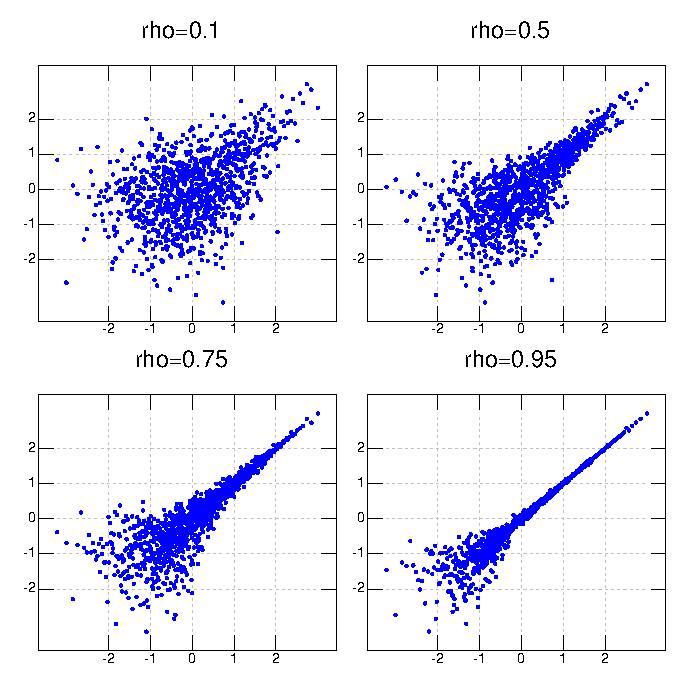
\includegraphics{fig3.eps}
\caption{Simulated values from \eref{chi1} if $\alpha_t\sim \chi^2_1$ with $F$ normal\ .}\label{fig3}
\end{figure}

\subsection{Pareto marginals}

The the inverse of the Pareto distribution is  
$$
F^-(u)= b\left\{(1-u)^{-1/a}-1\right\}\ ,\qquad 0<u<1\ ,
$$
where $a>1$ and $b>0$ are the parameters of the Pareto.  The mean of the distribution is $a/(b-1)$.  Thus with Pareto marginals the model becomes
$$
y_t=b\left\{(1-\check s_t)^{-1/a}-1\right\}\ ,\quad s_t=Z\alpha_t+\psi\cdot\eps_t\ , \qquad \eps_t\sim N(0,I)\ ,
$$
where $a$ and $b$ are vectors of parameters and the first equation is interpreted in an obvious componentwise sense.

\subsection{Other candidate marginal distributions}
Since $F_i^-$ maps numbers between 0 and 1 to real numbers it is convenient to think of them as
$$
1'a+\sum_i b_i\ln \frac{u}{1-u} = 1'a+\ln\prod_i\left(\frac{\check s_{it}}{1-\check s_{it}}\right)^{b_i}
$$
These have means $a_i$ and variances $b_i^2\pi^2/3$.

\section{Estimating loss distributions}

This leads to claim distribution.
\begin{equation}\label{loss}
c_t =\sum_{i=1}^p\frac{b_i}{(1-\check s_{it})^{1/a_i}}-1'b\ .
\end{equation}
Simulating this loss is a three step process:
\begin{enumerate}
  \item Simulating $N$ realizations of $s_t$.
  \item Computing the percentile ranks $\check s_t$.
  \item Combining the $\check s_t$ as in \eref{loss}.
\end{enumerate}
This formula is of independent interest. If $s_{it}$ is near 1, that is we are in the upper tail, then losses are likely to be huge.

Note that if $u$ is uniform then
$$
\frac{b}{(1-u)^{1/a}}
$$ is Pareto
In practice, for given parameter values, the losses $\ell_t$ and the loss distribution can be simulated.   This yields relevant percentiles.

\section{Time series structure}

Up to now it is assumed the $\alpha_t$ are independent random variables.  An alternative is where $\alpha_t$ has a time dependent structure.  A simple example is a geometric random walk
$$
\alpha_{t}=\e^{h_t/2}\ , \qquad h_{t+1}=h_t+\eta_t\ .
$$
$$
\alpha_{t+1}=(\eta_{t+1})^2
$$




\section{Connection to previous literature}
This setup \eref{gfac} is reminiscent of the usual factor model \cite{dnlawley1971fas} often employed to study the joint behavior of variables.  Similar to the ordinary factor analysis $Z$ spells out the way in which the heavy tailed factors manifest themselves into the components of $s_t$ and hence their percentiles $\check s_t$.

The formulation \eref{gfac} displays the obvious connection to state--space models \cite{Harvey:89}.  In terms of this latter model,  $\alpha_t$ is called the state of the system which manifest in the signal $s_t$.  The signal serves to determine the percentiles $\check y_t$ of $y_t$.   The model is completed by specifying the marginal distributions of $y_t$.

\section{Goodness of fit}

Suppose $n$  observations on a vector random variable $y$ denoted $y_1, y_2, \ldots, y_n$. The aim is to estimate the parameters in $Z$ and $\Psi$.   Suppose these two matrices depend on unknown parameters $\theta$ and $\rho$, respectively.

The first step in the estimation is to convert the $y_t$ to percentiles.  This is done either relative to a fitted marginal distributions $\hat F$ in which case $\hat F(y_t)$ is the vector of estimated percentiles, or by computing the percentile ranks 
$
\check y_t \equiv n^{-1}\ra(y_t)
$.
In the former case the estimated percentiles need not be exactly uniformly distributed although this does hold in the latter case.

Suppose we use the $\check y_t$.  Then according to the model $\check y_t=G(s_t)$ and 

You can plot the time series of percentile ranks.  Actually what you do is simulate a large number of 
Given a vector of actual or estimated marginal distributions $F$ the percentile ranks are
$$
\check y_{t} = F(y_t) \approx \frac{1}{n}\sum_{r=1}^n (y_r<y_t)\ ,\qquad t=1,\ldots,n\ .
$$
The right hand side are the estimated percentile ranks in the situation if there is no estimate of $F$, and $(y_r<y_t)$ is the vector of 1's and 0's indicating whether the corresponding component of $y_r$ is  than $y_t$ or otherwise.

The model states $\check y_t$ has the same distribution as $\check s_t$ where $s_t$ is  generated as in \eref{gfac}.  For given $\theta$ and $\rho$, the percentiles $\check s_t$ are estimated by simulating a large number $N$ of $s_t$ from \eref{gfac} and computing
$$
\check s_{t} \approx \frac{1}{N}\sum_{r=1}^N(s_{r}<s_{t})\ , \qquad t=1,\ldots,N\ .
$$
The distribution of the $\check s_t$ is compared to the distribution of the $\check y_t$.   Good estimates of $\theta$ and $\rho$ will lead to good correspondence between the outcomes $\check y_t$ and $\check s_t$.

One way to check whether the distribution of the $\check s_t$ is similar to that of the $\check y_t$ is to divide the unit hypercube into smaller volumes or cells indexed by $c$ and count the number of $\check y_t$ in each cell.   These are then compared to the expected number $e_c$ calculated for given $\theta$ and $\rho$ by simulating a large number of $s_t$ and calculating the corresponding $\check s_t$.  An appropriate choice for $\theta$ and $\rho$ is indicated by a low value of chi--squared goodness of fit statistic
\begin{equation}\label{chisq}
X^2\equiv \sum_c \frac{(o_c-e_c)^2}{e_c}\ ,
\end{equation}
where the $c$ sum extends over all cells.  In practice $X^2$ in  \eref{chisq} is numerically minimized  over a grid of values of $\theta$ and $\rho$.

\section{Estimating total loss quantiles}

Under the model \eref{gfac} it is easy to simulate the distribution of total loss given the parameters $\lambda$ and $\rho$.   For each of the $N$ simulated values of the state vector $s_t=Z\alpha_t+\Psi\eps_t$ the corresponding estimated loss is
$$
\ell_t = 1'(\hat F^-\circ \hat G)(s_t)=1'\hat F(\check s_t)\ ,
$$
where $1$ is a vector of ones and $\hat F$ and $\hat G$ are the vectors of estimated marginal distributions.   In particular $\hat G(s_t)=\check s_t$ where the latter is determined with reference to the $N$ simulated $s_t$.

Ranking the $\hat\ell_t$, $t=1,\ldots,N$ yields the $1/N$ quantiles of the loss distribution.   These quantiles are conditional on the estimated copula parameters in $\lambda$ and $\rho$ and the assumed or estimated marginals in $F$.  However under a suitably large sampling effort $N$, the quantiles will be independent of the approximation involved in $G$.


$$
\ell_t=1'F^-(\check s_t)\ , \qquad s_t=Z\alpha_t+\Psi\eps_t\ ,
$$
where $F$ is the vector of marginal distributions and $F^-$ the vector of componentwise inverses.  The marginal distributions $F$ is either specified analytically, or determined empirically.
 \begin{itemize}
   \item This case requires proper spanning of the actual losses. Suppose $y_t$ are the vectors of observed losses and $\check y_t$ the corresponding vector of percentile ranks.  Then the total loss distribution is that of the $\ell_r$, $r=1,\ldots,n$ where
$$
\ell_r = 1'y_r\ ,\qquad y_r \check = s_t\ , \qquad s_t=Z\alpha_t+\Psi\eps_t\ ,
$$
where the middle expression indicates the components of $y_r$ are chosen from the components of the available $y_t$ so that $\check y_r$ is as close as possible to $\check s_t$.  Thus in this case a large number of $s_t$ are simulated and converted to percentile ranks.   Each observed $y_r$ is then associated with a simulated $s_t$ with the same, or approximately the same, percentile rank.

   \item  In the case where $F_*$ is available (either the true marginal distribution or an estimate) then the distribution of losses is built up from
       $$
       \ell_t =1'F_*^-(\check s_t)\ , \qquad s_t=Z\alpha_t+\Psi\eps_t\ ,
       $$
       Thus in this situation a large number of $s_t$ are simulated from the model from which the percentile ranks $\check s_t$ are computed.   These $\check s_t$ are then used to compute $\ell_t$ corresponding to each simulation $t$.
 \end{itemize}




Suppose $y_t$ represents a vector of losses at time $t$ on each of $p$ classes of business.   Then $x_t\equiv 1'y_t$ is the total loss and of interest is the quantile of $x_t$ corresponding to the percentile $0<\pi<1$.  In applications typical values for $\pi$ are 0.95 and 0.99.

To estimate the quantile of $x_t$.

Consider first the two dimensional case.  Percentile $\pi$ in two dimensions is carved out of the unit cube as follows.  Suppose firstly $y_{2t}=0$.  Then $y_{1t}$ is the quantile corresponding to $\check y_{1t}=\pi$.

Suppose $F_*$ is vector or marginal distribution functions and consider for vector $0<u<1$
$$
x\equiv 1'F_*^-(u)\ .
$$
This is the loss when each line of business is at the percentiles given by $u$.  Taking the total differential yields
$$
\de x = 1'\de F_*^-(u) = \frac{-\de u_1}{f_1(y_1)}+\cdots +\frac{-\de u_p}{f_2(y_p)}\ ,
$$
where $y=F_*^-(u)$.  If $\de x=0$ and $p=2$ then
$$
\frac{\de u_1}{f_1(y_1)}=\frac{-\de u_2}{f_2(y_2)}\qquad\Rightarrow\qquad
-\frac{\de u_2}{\de u_1} = \frac{f_2(y_2)}{f_1(y_1)}\ .
$$
This is the slope of an iso--loss curve and is the rate at which the percentile rank $u_2$ must be changed when the percentile ranks $u_1$ is changed in order to maintain the same level of total loss.

Suppose the Pareto survival curve
$$
S(x) = \left(\frac{\theta}{x+\theta}\right)^{\alpha}
$$
This implies
$$
f(x)=\frac{\alpha S(x)}{x+\theta}\ , \qquad S^-(u)= \theta (u^{-1/\alpha}-1)\qquad\Rightarrow\qquad f\{S^-(u)\}=\frac{\alpha u^{1+1/\alpha}}{\theta}\ .
$$
Hence in this case
$$
\ln \left|\frac{\de u_2}{\de u_1}\right|= \ln \frac{\alpha_2\theta_1}{\alpha_1\theta_2} +\left(1+\frac{1}{\alpha_2}\right)\ln u_2-\left(1+\frac{1}{\alpha_1}\right)\ln u_1\ .
$$
Note if $\alpha_1=\alpha_2=\alpha$ then
$$
\ln \left|\frac{\de u_2}{\de u_1}\right|= \ln\frac{\theta_1}{\theta_2} + \left(1+\frac{1}{\alpha}\right)\ln \frac{u_2}{u_1}
$$



 The negative of the slope, $-\de u_2/\de u_1$ is the (marginal) rate of quantile substitution (MRS).  MRS depends only on the marginal distributions $F_*(u)$.
\newcommand{\s}{\sigma}

The elasticity of substitution is defined as
$$
\s (u_1,u_2)\equiv \frac{\de\ln(u_2/u_1)}{\de \ln (\mathrm{-\de u_2/\de u_1})}
$$
which is the percentage change in the relative size of the quantiles given a percentage change in the marginal rate of  substitution.


   It would be nice to be able have a functional form for the components of $F_*(u)$ so that RQS take a simple form.  That is we estimate some nice functional form



Suppose we have
\begin{equation}\label{ces}
    s(u) =\left( \sum_{i=1}^p a_i^{\frac{1}{\s}}u_i^{\frac{\s-1}{\s}}\right)^{\frac{\s}{\s-1}}\ .
\end{equation}
Then the $p$ marginal distributions are parametrized by the $p$ numbers $a_j$ and the constant elasticity of substitution $\s$.

To see the meaning of the $a_i$ note $s(0)=0$ while   $s(1)=\sum a_i^{1/(\s-1)}$ which is the maximum loss.  Further if $u$ is  all zeros except in component $i$ where it is $u_i$ then (\ref{ces}) reduces to
$$
y_i=F_i^-(u_i)=a_i^{1/(\s-1)}u_i\qquad\Rightarrow\qquad u_i=F_i(y_i)=a_i^{1/(1-\s)}y_i
$$
Thus $F_i(y_i)$ is linear in the tail up to some maximum point $y_i=a_i^{1/(\s-1)}$.  Note that the maximum of $\ln y_i$ is $(\ln a_i)/(\s -1)$.


Iso--loss lines can be easily constructed from

Given $u$ we can easily determine the total loss to which this corresponds $s=1'F^-(u)$.  By simulating from the copula of $u$ we can determine the frequency distribution of $s$.  In particular if $\Psi$ is the distribution of $s$ then $G(s)=G\{1'F_*^-(u)\}$ is uniform.  In other words
$G\circ 1'\circ F_*^-$ is a mapping from copula distributed $u$ to uniform random variables.

The rate of quantile substitution depends only on the relative magnitudes of the densities.  The rates are used to construct a iso--loss contours.   Integrating the density of copula above the iso--loss curve corresponding to $s$ yields the probability of exceeding the loss $s$.

A sampling scheme is as follows.
$$
s=1'\hat F_*^-(u)\ , \qquad u\sim C
$$
Alternatively to find out what quantile a given $s$ corresponds to, first construct the iso loss line corresponding to $s$.   Repeatedly draw $u$ and see the proportion of those $u$ for which $1'\hat F_*^-(u)$ exceed $s$.

An improvement is where we first select $u_1$ uniformly from $(0,1)$.   If $y_1\equiv F_1^-(u_1)>s$ then stop or alternatively if $F_1(s)>u_1$ then stop.  If not compute draw $u_2\sim u_2|u_1$ and $F_2(s-y_1)>u_2$ then stop.

the positive number $s-F_1^-(u_1)$.  This is the number $y_2=F_2^-(u_2)$ has to exceed in order for the sum to exceed ...   That is we want
$$
F_2\{s-F_1^-(u_1)\}
$$

Accept--Reject sampling can also be used.   We draw


Consider $p_1u_1+p_2u_2$ where $p_1$ and $p_2$ are prices.  The prices may represent the cost of reducing each of the quantiles.   To minimize $s$ subject to





In the two dimensional case.


The aim is, to find $\lambda$ and $\rho$  consistent with the observed percentile ranks $y_j^\#$.   This can be done as follows.




\section{Junk}
Thus we have $C_{\lambda,\rho}$ and our model is
$$
y\sim C_{\lambda,\rho}\circ F_*\ , \qquad y\sim F_*^-\circ C_{\lambda,\rho}
$$
Note the left hand side states how probabilities associated with $y$ are calculated, namely
$$
P(y\le\tilde y) = (C_{\lambda,\rho}\circ F_*)(\tilde y) \equiv C_{\lambda,\rho}\{F_*(\tilde y)\}\ ,
$$
while the right hand side indicates how one generates $y$: first you generate the uniforms according the copula, then you use these uniforms to interpolate out of the marginals: namely
$$
y = F_*^-(u)\qquad \mathrm{where}\qquad u\sim C_{\lambda,\rho}\ .
$$
Alternatively we can thus write the setup as
$$
y=F_*^-(s^\#)\ , \qquad s=\Lambda f + D\eps\ .
$$

\section{Connection to time series models}
A time series version of this is
$$
\check y_t=\check s_t\ , \qquad s_t=Z \alpha_t + \Psi u_t\ , \qquad u_t\sim N(0,I)\ , \qquad \alpha_t\sim \chi^2_1\ .
$$




These generated $s$ values are used to find synthesized $s(y_j)$ values corresponding to the $y_j$  such that $s^\#(y_j)=y_j^\#$.  We then measure
$$
\min_\psi \sum_{j=1}^n\|s_j-s(y_j)\|^2
$$


 and construct the empirical distribution of the percentile ranks $s_j^\#$, $j=1,\ldots,N$.  Corresponding to each $y_j^\#$, pick out
$s(y_j^\#)$, which is the generated $s$ with percentile ranks $s^\#$ closest to that of $y_j^\#$.
Then the log--likelihood of $(\lambda,\rho)$ based on  $y_j^\#$, $j=1,\ldots,n$ is
$$
\ell(\lambda,\rho) \approx \sum_{j=1}^n \ln f\{s(y_j^\#)|\lambda,\rho\}\ ,
$$
where here $f$










\section{Copula properties}

Consider a multivariate probability distribution $F$.  Define $F_*$ as the vector of marginal distributions derived from $F$.  In particular if $y\equiv(y_1,y_2,\ldots, y_p)$ then
$$
F_*(y) \equiv \left(
           \begin{array}{c}
             F(y_1,\infty,\ldots,\infty) \\
             F(\infty,y_2,\ldots,\infty) \\
             \vdots \\
             F(\infty,\ldots,\infty,y_p) \\
           \end{array}
         \right)\equiv \left(
           \begin{array}{c}
             F_1(y_1) \\
             F_2(y_2) \\
             \vdots \\
             F_p(y_p) \\
           \end{array}
         \right)\ .
$$
In other circumstances the vector of marginals $F_*$ is specified directly.

A copula is a probability distribution $C$ on the unit hypercube with uniform marginals.  Thus $C_*(y)=y$ for  $0\le y\le 1$ implying $C_*=1$.

The usefulness of copulas, arises as follows.  Consider a multivariate distribution $F$ and define the distribution generated with copula $C$ and given marginals $F_*$:
 \begin{equation}\label{Fx}
    F_C\equiv C\circ F_*\ ,
\end{equation}
Then $F_C$ is a joint distribution with $(F_C)_*=F_*$ since $F_C$ has marginals
$$
(C\circ F_*)(\infty,\ldots,y_i,\ldots,\infty)= C\{1,\ldots,F_i(y_i),\ldots,1\} = C_i\{F_i(y_i)\}=F_i(y_i)\ .
$$


Conversely given a joint distribution $F$ with marginals $F_*$ and $F_*^-$ as the componentwise inverse to $F_*$ define the copula generated from $F$ as
\begin{equation}\label{Cu}
    C_F\equiv F\circ F_*^-\ .
\end{equation}
Then $C_F$ is a copula since it has uniform marginals:
$$
(C_F)_i(u_i)=(F\circ F_*^-)(1,\ldots,u_i,\ldots,1)= F\{\infty,\ldots,F^-_i(u_i),\ldots,\infty\} = u_i\ .
$$
Every $F$ has a copula representation which is clear from
$$
F_{C_F}= C_F\circ F_*= F\circ F_*^-\circ F_*=F\ .
$$
Finally note
$$
C_C=C\ , \qquad C_{F_C}=F_C\circ (F_C)_*^-=C\circ F_*\circ  F_*^-=C\ .
$$

\section{Copula properties}
\begin{itemize}
    \item $C_*(y)=y$.  If $y\sim F_C$ then $F_*(y)\sim C$.  If $u\sim C_F$ then $F_*^-(u)\sim F$.
    \item  If $H_*$ is the componentwise  vector of univariate monotonic functions then
$$
C_{F\circ H_*^-}\equiv F\circ H_*^- \circ(F\circ H_*^-)_*^-=F \circ F_*^-\equiv C_F\ .
$$
Hence copulas are invariant to monotonic transformations.
    \item The density associated with $C_F=F\circ F_*^-$ is
    $$
    \frac{f\circ F_*^-}{\Pi (f_*\circ F_*^-)}\ ,
    $$
    where $f$ is the density associated with $F$ and $f_*$ is the vector of marginal densitities.  If $f=\Pi f_*$ (ie independence) then $f\circ F_*^-=\Pi (f_*\circ F_*^-)$ and the density is identically 1.
    \item The Gaussian copula with correlation matrix $R$ is the copula $C_{\Phi^R}$  where $\Phi^R$ is the Gaussian distribution with mean 0 and covariance matrix $R$. Since $R$ is a correlation matrix $(\Phi^R)_*=\Phi_*$, a vector of standard normal distributions, and $C_{\Phi^R}=\Phi^R\circ \Phi_*^-$.   The meta--Gaussian model is
\begin{equation}\label{metaG}
F_*(y)\sim C_{\Phi^R}\qquad\Leftrightarrow\qquad F_*(y) =\Phi_*(\eps)\ , \qquad \eps\sim N(0,R)\ .
\end{equation}
Matrix $R$ is estimated using the average cross product matrix of  the normits  $(\Phi_*^-\circ F_*)(y)$.
\item The meta--gamma model  is
$$
F_*(y)=\Gamma_\psi(1 \eta + \Psi\eps)\ , \qquad (\eta,\eps')'\sim \Gamma(\mu,\nu)\ ,
$$
where $\psi$ is a vector of parameters, $\Psi=\diag(\psi)$ and $\Gamma_\psi$ the vector of marginal distributions associated with $1\eta+\Psi\eps$.
\item  The Levy copula is $L$ such that $L_*(u)=u$.  Thus it is a copula on the unit hypercube suitable extended to $u>1$.
\item The independence and perfectly dependent copulas is defined as $\Pi\equiv\Pi\ 1_*$ and $\vee\equiv\min$ respectively, where $1_*$ indicates the vector of identity functions.  These arise as follows:
$$
C_{\Pi F_*}\equiv(\Pi F_*)\circ F_*^-= \Pi\ 1_*\ ,\qquad C_{\vee}=\ .
$$
The perfectly dependent copula implies a single source of noise:
$y=F_*^-1u$ with $u\sim U$
where $1$ is a vector of  identity functions of one variable.

\item  Any copula is ``symmetric" in the sense that if $C$ is the copula of 2D vector $u$ then it is also the copula of the $u$ with the components interchanged.  This follows since suppose the density associated with $C$ is $c$.   Then since $c(u_1)\equiv 1\equiv c(u_2)$,
$$
c(u_1|u_2) = \frac{c(u_1,u_2)}{c(u_2)} =c(u_1,u_2) =\frac{c(u_1,u_2)}{c(u_2)}= c(u_2|u_1)
$$

\item If $C$ is a copula then $C\circ (1-)$ is the ``survival" copula.  Here $(1-)$ is defined such that $(1-)u=1-u$.  To prove this result note that
\end{itemize}

\section{Factor copula models}
The simplest factor copula model is as follows. Given a vector of nonnegative weights $\psi\ge 0$, suppose $G$ is the distribution of
$$
1\eta+\Psi\eps\qquad\mathrm{where}\qquad \eta\sim\chi^2_1\ , \qquad \eps\sim N(0,I)
$$ with $\eta$ and $\eps$ independent and $\Psi=\diag(\psi)$.  Further suppose $G_*$ is the vector of marginal distributions associated with $G$.   Then $u\equiv G_*(1\eta+\Psi\eps)$ is a vector of uniform, albeit dependent, random variables. Hence the distribution of  $u$ is a copula.

In terms of this development we suppose $y$ is generated by the marginals $F_*$ and copula derived from $G$ if
$$
F_*(y) =  G(\Lambda f +\Psi\eps)\qquad\Leftrightarrow\qquad y\sim F_*^-\circ C_G \ .
$$
These steps make it clear how things are structured.  First, the factor scores are generated.  Then transformed to uniforms and finally transformed from the uniforms to the things in the tails.

\section{Generated practical copula structures}
To simulate the model for given $F_*$ and given $\psi$, we first generate the many values of the scores $1f+\Psi\eps$. These scores are then transformed to percentile ranks and these percentile ranks are used to pull out the corresponding values from the marginal distribution.

Initially suppose $f=\chi^2_1$.


 $G_*(1f+\Psi\eps)$ one first simulates $1\eta+\Psi\eps$ and then applies the  $G_*^\psi$.  However a simpler, more practical procedure is simply to simulate a large number of $1\eta+\Psi\eps$ and then compute empirical quantiles corresponding to each component.  Figure \ref{uv} displays realizations in the bivariate case for four different values of $\psi$.   In each case the first component of $\psi$ is zero while the second component is the given positive value.

   Each of these figures was generated as follows.
\begin{enumerate}
  \item For $t=1,\ldots,n=10000$ generate $\eta_t\sim\chi^2_1$ and $\eps_t\sim N(0,I)$ of order 2 and construct $\gamma_t\equiv 1\eta_t+\diag(\psi)\eps_t$, $t=1,\ldots,n$.
  \item Compute the quantiles associated with $\gamma_{it}$ for each $i=1,2$.
\end{enumerate}

\section{Wang article}

Suppose $x$ is a vector of losses (random).  Assume from $x$ you derive (componentwise) a vector of risk capitals $r(x)$ where $r$ works componentwise.   There are two rules for calculating capital:
\begin{itemize}
  \item Basel Accords: $\iota'r(x) = \sum_ir_i(x) =\sum_ir_i(x_i)$.
  \item US Insurance NAIC RBC: $\sqrt{\sum_ir_i^2(x_i)}$.
  \item Company models:  Individual probability distributions for a company's risks are quantified.  Then assuming a correlation matrix the aggregate loss distribution is calculated yielding percentiles etc.   The total economic capital is then distributed back to the business units according to
      $$
      \pi_i = \frac{\iota'R u_i}{\iota'R\iota}\ , \qquad \iota = \sum_i u_i
      $$
      where $u_i$ is a vector of zeros except in position  $i$ where it is 1.
\end{itemize}

Next states that yield spreads exaggerate default rates.  Goes on to posit the model for the price of risk $h_t$ where
$$
h_t = \hat\mu_t + \lambda_t\sigma_t\ ,\qquad \hat \mu_t = \mu_t + \eps_t\ , \qquad \cov(\eps_t) = (\partial\sigma_t) C(\partial\sigma_t)
$$
where $\lambda_t$ is a scalar stochastic process, $C$ is a correlation matrix and $\partial \sigma_t$ is the diagonal matrix formed from the standard deviation vector $\sigma_t$. Also $\mu_t$ is the true mean value of the loss: ie $\mu_t=\E(x_t)$.  Assume $\cov(\eps_t,\lambda_t)=0$ implying
$$
\cov(h_t) = (\partial\sigma_t) C(\partial\sigma_t) + \cov(\lambda_t)\sigma_t\sigma_t'
$$
\subsection{Corner tail correlations}
The proposed measure of tail correlation proceeds as follows.   take the percentile ranks and map to the z--scores ie $z_j=(\Phi^{-1}\circ F_*)(x_j)$.  Assuming $x_j$ is bivariate, write $\pi(\alpha)$ as the proportion of the $x_j$ falling in the lower corner.  The lower tail correlation is the solution for the off diagonal entry in the correlation matrix $R$ of
$$
(\Phi^R\circ\Phi^{-1})(1\alpha) =\E[\Pi \{\hat F_*(x_j)<1\alpha\}]\ .
$$
where $\E$ denotes the empirical expectation (ie fraction).  Why not try and find the optimal $R$.

\section{Copula factor model}

Suppose $\p$ computes the ``uniforms" of a random variable. Then for any monotonic transform $f$, $\p\circ f=\p$ and hence $\p\circ \p=\p$.  Further for a monotonic decreasing function $\p\circ f = 1-\p$ implying $\p\circ (1-\p) = 1-\p$.  Also $\p\circ -=1-\p$.

 And suppose $\psi$ a vector of weights.  Then $y$ is said to be generated by the copula factor model if
$$
\p(y_t)= \p(\Lambda f_t+\Psi\eps_t)\ , \qquad f_t\sim\chi^2_\nu\ \mathrm{or}\  t_\nu\ , \qquad \eps_t\sim N(0,\sigma^2I)\ ,
$$
where $\Psi$ is a diagonal matrix with diagonal $\psi$.
Without loss of generality assume the first component of $\psi$ is zero.

\subsection{Different specifications}

Here show the effect of different $\Lambda$ and $\Psi$ and perhaps replacing $\Lambda f_t+\Psi\eps_t$ by eg $\Lambda(f_t)+\Psi\eps_t$.

\subsection{Rank correlation}

Suppose $\R(y_t)$ is the rank correlation matrix of $y_t$: that is $\R(y_t)\equiv \cor\{\p(y_t)\}$

\subsection{Estimating the copula factor model}
Consider $\hat\p(y_t)$.  If we know the cdf $\p_x$ of $x_t\equiv\Lambda f_t+\psi\eps_t$ then $\hat x_t=(P_x^-\circ \hat P)(y_t)$.  However we don't know $\p_x$.   However simulate $x_s$, $s=1,\ldots,N$ and reorder the simulated components of $x_s$, $s=1,\ldots n$ to yield $\tilde x_t$ so that $\hat\p(\tilde x_t)=\hat\p(y_t)$.  In other words we order the simulated components of $x_s$ according to the order specified in $y_t$.

What is the relationship of this to finding $\psi$ such that the rank correlation is preserved.  In this we simulate $x_t$ from the model and adjust $\psi$ till we get a rank correlation for the $x_t$ equal to the observed rank correlation.  Obviously this procedure cannot tell us anything about order of things.

So we use the procedure of the last paragraph to find $\psi$.   Then for the given $\psi$ we simulate $x_s$, $s=1,\ldots,n$ and in turn $\tilde x_t$.   We use the $\tilde x_s$ to infer about the $f_t$.


Given the estimate $\tilde x_t$ of $x_t=\Lambda f_t+\Psi\eps_t$ we can do a PC analysis on $\tilde x_t$.

   Then $\hat\p(\tilde x_t)=\hat\p(y_t)$ and $\tilde x_t$ is our estimate.


 and in particular $+/\hat\p(y_t)$.   If we know
$\Lambda f_t$ then take



Consider the the principal components of $\hat\p(y_t)$.   These
pick up the major directions of variation.
The vector $\psi$ is estimated by the following steps:
\begin{enumerate}
  \item Calculate the principal components of $\hat \p(y_t)$ to yield say $UDU'$.
  \item If $u$ is the first column of $U$ compute $u'\hat \p(y_t)\}\approx \p(f_t)$.  This the vector of weights.
  \item Minimize
\end{enumerate}


Given $\psi$ and hence $\Psi$ we simulate $1f_t^s+\Psi\eps_t^s$ and reorder each scalar series in  each simulation to yield $x_t^s$ such that $\hat \p(x_t^s)=\hat \p(y_t)$. Note that $x_t^s$ is $y_t$ interpolated back into the EDF of $1f_t^s+\Psi\eps_t^s$.



\subsection{The two variable case}

To illustrate estimation consider first the case where $y_t$ is two dimensional $\Lambda=1$.   Suppose $r$ is the correlation between the ranks the two components in $\hat\p(y_t)$ -- that is the rank correlation between the components in $y_t$.  Then we want to estimate $\psi$ subject to
$$
\cor\{\hat\p(1f_t+\Psi\eps_t)\}=\cor\{\hat \p(y_t)\}\ .
$$
Notice the correlation decreases with $\psi$.   So we simulate $1f_t+\Psi\eps_t$ and compute $\cor\{\p(1f_t+\Psi\eps_t)\}$.  Then

 Put $y$ as the $2\times n$ vector of $y_t$, $t=1,\ldots,n$.  Write $x_t=\Lambda f_t+\Psi\eps_t$ and without loss of generality $\Psi=\diag(0,1)$. For given $s=\sigma$ generate a simulated path of $x_t$ denote $x^s$.  Note $x^s$ is $2\times n$.  Rank each row of $x^s$ according to the ranks of $y$ denoted $\tilde x^s$ and redefine $s$ as  the standard deviation of   $\Delta \tilde x^s$ where the latter subtracts the first row from the second.  Cycle through this procedure as in Gibbs sampling to get a distribution of $s$.  This is the posterior distribution of $\sigma$.


Then calculate the units of each component in  $y_t$ and calculate its value in the empirical cdf of the corresponding component of $x_t$.   To achieve this rank, for each $i$ the  $x_{it}$, $t=1,\ldots,n$ according to the ranks of  $y_{it}$, $t=1,\ldots,n$.  Suppose this yields $\tilde x_t$.  This is equal to $ \eps_{2t}$.  So take the standard deviation of so as to get an estimate of $\sigma$.


 Thus the joint distribution is generated with the meta--gamma copula $C^\psi\equiv G^\psi\circ (G_*^\psi)^-$.

Maybe the model should be changed to something like this
$$
F_*(y) = H_*[1\Phi^-\{G(\eta)\}+(\partial\psi)\eps]\ , \qquad \eta\sim\chi^2_1\ , \qquad \eps\sim N(0,I)\ .
$$

\subsection{Estimation of copula parameters}
  Estimation and testing consists of the following steps:
\begin{enumerate}
  \item Compute the empirical cdfs $\hat F_*(y)$ and the percentile ranks $u_t=\hat F_*(y_t)$.
  \item Draw $\eta_i\sim \chi^2_\nu$ and $z_i\sim N(0,1)$ and form $w_i=1\eta_i+(\partial \theta)z_i$ for $i=1,\ldots,N$. Use the results to form an empirical estimate of $G_*^\theta$
  \item Use these to form an empirical estimate of $v_t(\theta)=G_*^{\theta-}(u_t)$.
  \item Compute
  $$
  \eps_{t}(\theta)\equiv \frac{v_{2t}(\theta) - v_{1t}(\theta)}{\theta}\ , \qquad t=1,\ldots,n\ .
  $$
  \item Compute the log--likelihood
  $$
  \ell(\theta) = \sum_{t=1}^n\eps_t^2(\theta)
  $$
  \item Choose $\theta$ such that $\ell(\theta)$ is minimum
\end{enumerate}

Here are some assertions I think are true about the meta--gamma.
\begin{itemize}
  \item The means on the $\eta_i$ or $\eps_i$ should not make a difference since we are transforming to percentiles.  Or maybe it is just the relative means or something.
  \item By tuning the gamma's we can pretty much describe any chi-squared/normal behaviour
  \item The sum of independent gamma's is gamma so we can easily figure out $G_\psi$ etc.
  \item If $\psi\rightarrow 0$ then the components of $y$ approach perfect dependence.
  \item If $\psi\rightarrow \pm\infty$ then the components of $y$ approach independence.
\end{itemize}


\section{Weibull losses}

Suppose the Weibull distribution function
$$
u=F(y)=1-\exp\left\{-\left(\frac{y}{\alpha}\right)^\beta\right\}\qquad\Rightarrow\qquad
F^-(u) = \alpha\left\{-\ln(1-u)\right\}^{1/\beta}\ .
$$
indicating that if $u$ is uniform then the right hand transformation is Weibull.
With this specification
$$
s(u) = \sum\alpha\left\{-\ln(1-u)\right\}^{\frac{1}{\beta}}\ ,
$$
Further note the density of corresponding to $F(y)$ is
$$
f(y) = \frac{\beta}{\alpha} \exp\left\{-\left(\frac{y}{\alpha}\right)^\beta\right\}\left(\frac{y}{\alpha}\right)^{\beta-1}\ = \frac{\beta}{\alpha}\left(\frac{y}{\alpha}\right)^{\beta-1}\{1-F(y)\}.
$$
implying the product out the front is the hazard.


Further.
$$
\de s = \sum\frac{\de u}{f\{F^-(u)\}}= \sum \frac{\alpha\left\{-\ln(1-u)\right\}^{\frac{1}{\beta}-1}}{\beta(1-u)}\ \de u\ .
$$
which defines the iso--loss curves.

In practice the parameters $\alpha$ and $\beta$ are estimated for each marginal distribution $F_i(y_i)$.  The mean and variance associated with the marginal distribution $i$ are then
$$
\alpha\Gamma\left(1+\frac{1}{\beta}\right)\ , \
\qquad \alpha^2\left\{\Gamma\left(1+\frac{2}{\beta}\right)-\Gamma^2\left(1+\frac{1}{\beta}\right)\right\}
$$



\section{Open question}

We note that $s(u)=\sum F_i^-(u_i)$ for some appropriate functions $\phi_i$.  The question is whether we can structure things such that this sum is nice.   One procedure is where we first choose $u_1$ uniformly and compute $F_1^-(u_1)$.  Next choose $u_2\sim u_2|u_1$ and compute $F_2^-(u_2)$.  Or we can just do the Gibbs sampling trick where we take $u_1|u_2$ then the other way round.

\section{Logistic losses}

Suppose
$$
s(u) = \sum \frac{\alpha u^\beta}{1-u^\beta} = \sum\frac{\alpha}{u^{-\beta}-1}
$$

\section{Iso--loss curves}





\section{Estimation in old notation}
To estimate $\lambda$ take the observations $y$ and initially transform to the quantiles
$$
u\equiv F_*(y) = G_\lambda(\chi_1^2+\lambda\cdot\eps)\ .
$$
Next, for given $\theta$ transform $u$ as
$$
G_\theta^-(u) = (G_\theta^- \circ G_\lambda)(\chi_1^2+\lambda\cdot\eps)\approx (G_\theta^-\circ G_\lambda)(\chi_1^2) + (G_\theta^-\circ G_\lambda)'(\chi_1^2)\lambda\cdot\eps\ .
$$
If $\theta=\lambda$ then this reduces to $\chi_1^2+\lambda\cdot\eps$ which has the known distribution. Hopefully things are invariant to the base category.

In this formulation $\lambda$ is unknown.  To estimate it proceed as follows:


If (\ref{ge}) holds $\hat\eps_t(\lambda)\sim N(0,I)$.  So the aim is to find $\theta$ such that

\section*{Generalizations}
More generally suppose
\begin{equation}\label{ge2}
y=(F_*^-\circ G_\lambda)(X\chi_1^2+H\eps)\ , \qquad \eps \sim N(0,I)
\end{equation}
To estimate we


\section*{Bivariate copulas}
In the following $X$ and $Y$ are scalar random variables.   The aim is to synthesize a bivariate copula with required properties.
\begin{enumerate}
  \item Consider
  $$(G_{X+Y}\circ G_X^-)(u) \equiv G_{X+Y}\{G_X^{-}(u)\}\ .
  $$
  This is the quantile in the $X+Y$ distribution if $X$ is at quantile $u$  in the $X$ distribution and $Y=0$.
      Thus if $G_Y(0)=0$ (ie $Y\ge 0$) it is the minimum quantile of $X+Y$ if $X$ is at quantile $u$ of the $X$ distribution.
  \item  Suppose $X$ and $Y$ are independent chi--squareds each with 1 degree of freedom.   Then $X+Y$ is chi--squared with 2 degrees of freedom.   Hence $(G_{X+Y}\circ G_X^-)(u)$ is the chi-squared 2 degrees of freedom distribution evaluated at quantile $u$  of the chi-squared 1 degree of freedom distribution.
  \item  Suppose $X\sim\chi_1^2$  and $Y\sim N(0,\sigma^2)$.   Then $(G_{X+Y}\circ G_X^-)(u)$ is the $\chi^2_1+ N(0,\sigma^2)$ distribution evaluated at quantile $u$ of the $\chi^2_1$ distribution.
  \item Consider
  $
  G_{X+Y}\{G_X^-(u)+G_Y^-(v)\}
  $.
  This the quantile of $X+Y$ when $X$ is at quantile $u$ and $Y$ is at quantile $v$.

  \item  Consider $G_{X+Y}\{G^-_X(u)+Y\}$.  This is a random variable -- the quantile in the $X+Y$ distribution when $X$ is at quantile $u$ of the $X$ distribution.  Further
      $
      \E\left[ G_{X+Y}\{G^-_X(u)+Y\}\right]$ and $Var\left[ G_{X+Y}\{G^-_X(u)+Y\}\right]$ are the
      expected value and variance of the quantile in the $X+Y$ distribution if $X$ is at quantile $u$ in the $X$ distribution, respectively.

  \item  Suppose $X\sim \chi^2_1$ and $Y\sim N(0,\sigma^2)$.  Then
      $$
      \E[G_{X+Y}\{G_{X}^-(u)+Y\}]=u\ , \qquad Var[G_{X+Y}\{G_X^-(u)+Y\}]=
      $$
      To prove the first relation, note that
      $$
      P\{G_X^-(u)+Y<y\}=P(Y<y-G_X^-(u)\} = G_Y\{y-G_X^-(u)\}\ .
      $$
      that is a shifted version of $G_Y$.
\end{enumerate}
\subsection*{Runoff triangles and copulas}

Let $L_k$ be the liability distribution associated with runoff triangle $k$.   Suppose the joint distribution is modelled with a copula $C(u,v)$.  Thus the joint distribution of $(X,Y)$ is
$$
y\sim C\circ F_*
$$
Want $\iota'y$.  Let's think of things in two dimensions:
\begin{enumerate}
    \item Draw $u\sim C$ and
    \item Put $y=F_*^-u$
    \item Determine $y\sim F_*^-u$
    \item AHP for determining a copula
    \begin{enumerate}
        \item For each $u$ give probability distribution of $v$
        \item Draw $u_1\sim U$, $u_2\sim C_{2|1}$
        \item $y_1=F_1^-u_1$, $y_2=F_2^-u_2$.
    \end{enumerate}
\end{enumerate}


\subsection*{AHP with copulas}

Suppose $0\le u \le 1$ is given and let $U_1$, $U_2$ and $U_3$ be risk quantiles.  Suppose we know $U_1>u$.   We now ask how much more likely this makes $U_2>u$ and $U_3>u$.  Similarly if $U_2>u$ how much more likely does this make $U_1>u$ and $U_3>u$? In tabular format:

If $U_1>u$ what is the probability of:


\begin{tabular}{|c|c|c|c|c|c|}
  \hline
  % after \\: \hline or \cline{col1-col2} \cline{col3-col4} ...
  $P(U_1>u)$ & 0.5 & .25 & 0.10 & 0.05 & 0.025 \\
  \hline
  $P(U_2>u|U_1>u)$ & 1 & 1 & 1 & 1 & 1\\
  $P(U_3>u|U_1>u)$ & 0.5 & 0.25 & 0.10 & 0.05 & 0.025\\
  \hline
\end{tabular}
\\\\
This table indicates $U_2$ is perfectly dependent while $U_3$ is independent.
Since
$$
P(U_2> u|U_1> u) =\frac{P(U_2>u, U_1>u)}{P(U_1>u)} = \frac{P(U_1>u|U_2>u)P(U_2>u)}{P(U_1>u)}=P(U_1>u|U_2>u)\ ,
$$
it makes no further sense to ask the question the other way round.

\subsection*{Conditional Probability}

We have a risk vector $y$.   Define $u=F_*(y)$.   Then the marginal distributions of $u$ are uniform.   Next choose $u_1$.   We then have an effect on the conditional distributions of the remainder.   Hence construct $F_*(u|u_1)$ which again have uniform marginals, albeit of one dimension less.   The advantage is that if the effect of $u_1$ is simple on all the uniform marginals then we can keep track of everything and hopefully

\subsection*{Example copulas}

\subsubsection{Clayton} This depends on a single parameter $\delta$  and is defined as
$$
C(u)\equiv\left(\Sigma u^{-\delta}-d+1\right)^{-1/\delta}
$$
It is the distribution of
$$
u=\left\{1-\frac{\ln(v)}{\gamma}\right\}^{-1/\delta}
$$
where $\gamma \sim \Gamma(\delta^{-1},1)$ and $v\sim U^d(0,1)$.
In the last step things are done componentwise.

\subsubsection{Gumbel}
This also depends on a single parameter $\delta$ and is defined as
$$
C(u)\equiv  \exp\left[\left\{-\Sigma (-\ln u)^{\delta}\right\}^{1/\delta}\right]\ , \qquad \delta\ge 1\ .
$$
It is the distribution of
$$
u= \exp\left\{- \left(-\frac{\ln v}{s}\right)^{1/\delta}\right\}\ ,
$$
where $s\sim Stable$ and $v\sim U^d(0,1)$.

\subsection*{Problem}

Note that for a bivariate copula $f(v|u)=f(u,v)/f(u)=f(u,v)=f(u|v)$.  Choosing $u\sim f(u)$ and then $v\sim f(v|u)$ produces a draw $(u,v)\sim f(u,v)$.  But how do we constrain



So why does

One distribution is the beta distribution
$$
    f(v|u)=cv^{\alpha-1}(1-v)^{\beta-1}\ , \qquad \E(v|u)=\frac{\alpha}{\alpha+\beta}\ , \qquad \cov(v|u)=\frac{\alpha\beta}{(\alpha+\beta)^2(\alpha+\beta+1)}\ ,
$$
where $\alpha>0$ and $\beta>0$.  Now we want to make $\alpha$ and $\beta$ a function of $u$.  A way of doing this is to put $\alpha-1=-a\ln(u)$ and $\beta-1=-b\ln(1-u)$ to yield
$$
\ln\{f(v|u)\}=c-a\ln(u)\ln(v)-b\ln(1-u)\ln(1-v)=\ln\{f(u|v)\}\ .
$$
where $a>0$ and $b>0$.  Since $0<u<1$  then $\alpha>1$ and $\beta>1$.

Now $0<x<1$ and hence consider $\alpha=x/(1-x)$ implying $\alpha>0$.   Then $\alpha-1=(2x-1)/(1-x)$.  Note when $x=1/2$ then $\alpha-1=0$.




So suppose $\beta=1$
$$
f(y|x)= cy^{(2x-1)/(1-x)}\ .
$$
When $x=0.5$, $f(y|x)=1$.  As



Point is to relate $\alpha$ and/or $\beta$ to $x$, the conditioning variable.  When $x$ increases we want the mean to increase and vice versa.  So maybe make $\alpha=x/(1-x)$, $\beta=1$ in which case $\alpha-1=1/(x-1)$ and
$$
f(y|x)=cy^{1/(x-1)}
$$

  However further useful information is provided by $P(U_3>u|U_2>u)$. Natural questions that arise are:
\begin{itemize}
    \item Is the fact that we are conditioning both on $u$ important?
    \item What are the critical $u$ points to be considered?
    \item How do we measure consistency of choice across the different combinations?
    \item If we do have tables as above how do we combine them?
\end{itemize}

Combining tables.

Sampling scheme:
\begin{itemize}
    \item Select random $U_1$ from the uniform
    \item Find max table $u$ such that $U_1>u$ in the table
    \item With the table probability select $U_2$
\end{itemize}

Thus if it makes it $x_u$ times more likely then since $P(U_2>u)=1-u$ then
$$
P(U_2> u|U_1> u) = x_u(1-u)\ , \qquad P(U_2\le u|U_1> u) = 1-x_u(1-u)\ .
$$
Thus
$$
\frac{P(U_2> u|U_1> u)}{P(U_2\le u|U_1> u)}=\frac{x_u(1-u)}{1-x_u(1-u)}\ .
$$

\subsection*{Mortality smoothing with copulas}

Suppose $Y$ is a matrix of mortality measurements with rows indicating age $i$ and columns time $t$.   Define column vectors $y_t$ and $y_i$ as column $t$ and row $i$ of  $Y$, respectively.  There are two ways of smoothing the matrix $Y$:
\subsubsection{Age copula}  The copula $C$ models correlation across age and $y_t=F_*^-u_t$ where $u_t\sim C$. Age specific behavior across time defines the components of $F_*$ and are estimated from the ergodic average $\hat F_*(s) =\Ex[y_t<s]$.
Special cases are:
    \begin{enumerate}
        \item Time profiles the same for each age: $F_*=1\odot h$ where $h$ is a scalar function and estimated as $\hat h(s)\equiv\Ex\{\hat F_*(s)\}=\Ex\{\Ex[y_t<s]\}$ where the outer expectation is the ensemble, across age, average.
        \item \label{pd} Perfect dependence across age.  This implies all the component time series in $y_t$ are driven by a single source of noise: $u_t=1v_t$ with $v_t\sim U$.
        \item \label{ind} Independence across age implies $u_t\sim \Pi$.  This model invokes the unlikely assumption that each age moves independently over time.
        \item   The meta--Gaussian model correlation matrix $R$ models the contemporaneous correlation between ages with $\hat R=\Ex(z_tz_t')$ where the $z_t$ are the normits $z_t\equiv(\Phi_*^-\circ F_*)y_t\sim\Phi^R$.  Generally the correlation between close ages is  higher.   An extreme case is where the correlation between ages $i$ and $j$ is $\rho^{|i-j|}$ for $0\le\rho\le 1$.  The case $\rho=1$ is equivalent to \ref{pd} while $\rho=0$ to \ref{ind} above.
    \end{enumerate}

    \subsubsection{Serial copula} The copula $C$ models serial correlation and $y_i=F_*^-u_i$ where draws $u_i\sim C$ correspond to different ages. Time specific mortality curves are the components in $F_*$ and are estimated from the ensemble (age profile) average $\hat F_*(j)\equiv\Ex[y_i<j]$.
Special cases are:
\begin{enumerate}
    \item Age profiles are the same across time.  This  implies each marginal in  $F_*$ is the same: $F_*=1\odot h$ where $h$ is univariate and $(1\odot h) y_i$ applies $h$ componentwise.  Thus $y_i=(1\odot h)^-u_i=(1\odot h^-)u_i$.  Function $h$ is estimated from the ergodic average of the empirical ensemble (age profile) distributions
$
\hat h(j)\equiv \Ex\{\hat F_*(j)\}=\Ex\{\Ex[y_i<j]\}
$ where the outer $\Ex$ works across the components of the vector.
    \item Perfect serial dependence implies $u_i=1v_i$ where $v_i\sim U$. Combined with a single age profile yields $y_i=(1\odot h^-)1v_i=1h^-v_i$.
    \item Matrix $R$ in the meta--Gaussian model is a serial covariance matrix, estimated from the normits $z_i\equiv(\Phi_*^-\circ F_*)y_i\sim \Phi^R$ as
$
\hat R = \Ex(z_iz_i')
$.
With a fixed mortality curve $z_i=\{\Phi_*^-\circ(1\odot h)\}y_i$ implying each component of $y_i$ is transformed with a fixed $h$.

\item    With the meta--Gaussian model the stationary AR(1) case  is where entry $(t,s)$ of $R$ is $\rho^{|t-s|}$ with $0\le\rho\le 1$.
Estimate $\hat\rho$ is derived from $\hat R$ by averaging the first off diagonal.
\end{enumerate}
Which copula modelling is likely to be more appropriate?  Copulas are preferred for variables which have distinct marginal behavious.

\subsubsection{Modelling age at death}

Let $F_t(i)$ be the age--at--death distributions at time $t$ and from this define $F_*$.  Thus $F_*$ is a vector of marginals corresponding to different points of time.  Corresponding to $y_i=F_*^-u_i$ with $u_i\sim C$ write, for each age $i$,  $u_i$ as the vector with components $F_t(i)$.  A copula $C$ serves to model dependence across age.

The above approach serves to define $u_i$ from the physically constructed age at death distribution, not actual deaths.   Of course the physical age--at--death distribution


\subsubsection{Connection to usual studies}

The distribution of age--at-death in a given year is
$$
F(y)=P(Y<y)= \sum_x P(Y<y|X=x)P(X=x) = \int_x F(y|x)f(x)
$$
Differentiating with respect to $y$ implies the density is
$$
f(y) = \int_x f(y|x)f(x)
$$
$$
 F(y|x)F_X(x)] - \int_xf(y|x)F_X(x)
$$
\subsubsection{Mortality smoothing across time}

Time dependence is introduced by assuming
$$
N_* y_t=Z\alpha_t+G\eps_t\ , \qquad \alpha_{t+1}=  T\alpha_t + H\eps_t\ .
$$
where $N_*\equiv \Phi_*^-\circ F_*$.  Hence the steps in this process are that we first construct the  normits $N_* y_t$ from each of the ages over time. We then fit a standard state space model to these normits.   But there must be a cycle here since the normits are estimated over time. Given a forecast $\hat z_t$ of the normits the forecast of $y_t$ is $\hat y_t=N_*^-\hat z_t$ where $N_*^-\equiv (\Phi_*^-\circ F_*)^-=F_*^-\circ\Phi_*$

An alternative is to define $N_+=\Phi_*^-\circ F_+$ where $F_+$ computes the quantiles of all the available data considered as one group.  Thus the measurement equation becomes $N_+y_t=Z\alpha_t+G\eps_t$.


A very simple model is
$$
N_* y_t=1\alpha_t+G\eps_t\ , \qquad \alpha_{t+1}=  \rho\alpha_t +\eta_t\ .
$$

\subsection*{BvN}

Theorem 1: The Birkhoff - von Neumann Theorem [Marcus (1960), pg. 215]
A doubly stochastic matrix A can be expressed as  , where   are nonnegative real numbers summing to 1 and   are permutation matrices.

Therefore any copula can be discretized and represented in matrix form based on the partition into   regions of equal size. Then, this matrix can be decomposed into linear combination of permutation matrices which can enhance the understanding of dependence structure and help to form a basis for multivariate data analysis. In the following sections we will set up BvN decomposition and copula connection, study the dependence bones and skeletons, discuss implications of the decomposition and generating copulas, and propose an approach to decompose copulas.


\subsection*{Power copulas}

Suppose $C$ is a copula.  For positive integer $p$ consider $C^p$.  This is a distribution on the unit hypercube.   The marginals are not uniform.   However we can construct the copula
$$
C^{(p)}\equiv C^p\circ C^{p-}_*
$$
What is the dependence structure here?  The procedure is thus:
\begin{itemize}
    \item Choose a given copula $C$.  For example $C=\Phi^R\circ\Phi_*^-$
    \item Power it.  For example $C^2=(\Phi^R\circ\Phi_*^-)^2$.  Note powering it means take the appropriate pointwise power not taking the function twice.
    \item Turn the powered version into a copula.
    \item Use the copula to model dependence.
\end{itemize}

\subsection*{Tail correlation}

We want an effective method to construct the correlation in the tail of  a distribution.   For example when dealing with the Gaussian distribution there is a single correlation that describes the strength of the relationship no matter where you are in the distribution.  How can we model the situation where there is more correlation in the tails?  Here is a try.  Think of the bivariate situation.  Divide the unit square into smaller squares.  In each square we correlate the normits of the quantiles.  Thus in each little square we have a bivariate normal and we compute the correlation.   To get the overall correlation we correlate the correlations.

Is this effective?  One way to think about things is to think about
$$
\tau(x,y)\equiv P(X>x|Y>y) = \frac{P(X>x,Y>y)}{P(S>y)}= \frac{S(x,y)}{S(y)}
$$
What is a smooth way of perturbing the normal to get more emphasis in the tail.  One way of doing this is to think of the distribution on each margin and then multiply by another distribution
$$
G\circ F
$$
Call $G$ the ``tail emphasizer."  In the extreme for example we can have $G$ as a step function with knot $\kappa$. Then result is a distribution which places a discrete mass at the knot and then as usual.  What if we take a ramp function...

Note that a copula is a function of many variables and returns a probability.  So you can't apply a copula repeatedly.  What happens if you take a copula $G$ and and generate a second copula from it.   That is you construct $C_C\equiv C\circ C_*$.  But the marginals $C_*$ of $C$ are uniform.   Hence $C_C=C\circ I=C$



What about taking a Gaussian copula and applying it repeatedly?   For example $G\equiv \Phi^R\circ\Phi_*^-$ is the Gaussian copula with correlation matrix $R$.  Using    What about $G^p$.  Note that $G$ is a copula.  Hence it takes probabilities to probabilities.   Thus $G^p$ is a copula for any integer $p$.   Note $G^0=I$, the uniform copula.

\subsection*{Survival copulas}

Copulas are typically thought of as the joint distribution on the square.  Alternatively let $S$ denote a survival function:
$$
S(y)=P(Y>y)
$$
We can then think of a survival copula on the square.  Thus a survival copula is a survival function on the unit cube with uniform marginals. Note for positive random variables $S(0)=1$ and $S(y)\rightarrow 1$ as $y\rightarrow\infty$.

Suppose $y\sim S$, indicating $y$ is a random vector with survival function $S$. Consider the ``survival" transform
$$
P\{S(Y)>y\} = P\{Y<S^-(y)\}=1-S\{S^-(y)\}=1-y
$$
Thus let $D$ be a survival copula on the unit hypercube with uniform marginals and $S_*$ a vector of survival marginals and define
$$
S_D\equiv D\circ S_*\ , \qquad D_S\equiv S\circ S_*^-
$$


\subsection*{Total liability distribution}

Consider
$$
\phi(s)\equiv P(\iota'F_*^-u\le s)\ , \qquad s_\alpha=\phi^-(\alpha)\ ,
$$
where $u\sim C$ and where $0\le\alpha\le 1$ is given.
What is a good way of estimating $F(s)$?   Further what is a good way of determining $s_\alpha$ given $\alpha$?  For example we may wish to estimate $s_{\alpha}$, corresponding to $\alpha=0.75$, the 75th percentile.

One approach is to repeatedly sample $u\sim C$ and hence $\iota'F_*^-u$.  These realizations are transformed to quantiles and in turn the quantiles are used to define  $s_\alpha$.

If we are interested in say the $\alpha$ quantile then hopefully we need only consider $u$ in the triangular pyramid of points lying above

Also important is the copula to be used.  What is a good copula?

Can we simplify.   For this purpose look at the 2D case and consider the point $(u,v)$ and suppose the quantile associated with this point insofar as the sum is concerned is $\alpha$.  Suppose we move $x$ to $x-\delta$ where $\delta>0$.   At the same time we move $y$ to $y+\delta$ and hence the sum stays the same.   The change in quantile in the $x$ distribution is  from $u=F_X(x)$ to $F_X(x-\delta)\approx F_X(x)-\delta f_X(x)=u-\delta f_X(x)$.  That is the change in the quantile is approximately $-\delta f_X(x)$.   Similarly the change in the $y$ quantile is approximately $\delta f_Y(y)$.  Thus the relative change in the $y$ quantile to that in the $x$ quantile is
$$
-\frac{f_Y(y)}{f_X(x)}\ .
$$

Fix $s>0$ and consider $\Omega_s=\{(x,y): x+y\le s\}$.  Clearly $(s,0)\in \Omega_s$.  Want $F_* (\Omega_s)$, the quantile set corresponding to $\Omega_s$.  Note
$$
F_*(\Omega_s)=\{u: \iota'F_*^- u\le s\}\ .
$$
What does this set look like?  Here we look at the 2D situation.   First consider (in 2D) $(u_s,v_s)=F_*^-(s,s)$.  These are the intercepts points, ie the quantiles in the marginal distributions that yield $s$.  Hence  $(u_s,0)$ and $(0,v_s)$ are in $F_*(\Omega_s)$.  Moving from $(0,s)$ to $(\delta,s-\delta)$ keeps us in $\Omega_s$.   The corresponding movements in $(u,v)$ space is from $(0,v_s)$ to $(\delta f_X(0), v_s-\delta f_Y(s))$.  Thus the slope is $-f_Y(s)/f_X(0)$.

The above argument can be generalized to any point when moving from $(u,v)$, presumed to be such that the corresponding $x+y=s$.  The change in $v$ relative to a change in $u$ is $-f_Y(x-s)/f_X(x)$.  Hence the boundary is defined by the differential equation
$$
\partial v=\frac{-f_Y\{F_X^-(u)-s\}}{f_X\{F_X^-(u)\}}\partial u\ ,
$$
with starting condition $(0,F_Y^-(s))$.

Once we have the boundary then we sample repeatedly from the copula and check if the sampled point lies on the right side of the boundary.   If so we count 1 and otherwise 0 and averaging we determine the quantile of $s$.  Alternatively we determine say the $\alpha$ quantile in $F_Y$ called $y_\alpha$ say.  We then use the above differential equation to define the boundary using $y_\alpha$ in place of $s$.  We repeatedly sample from the copula and check if we are on the right side of the boundary and count 1 or 0.   Averaging the 1's leads to the quantile of $y_\alpha$.  Generally expect that the quantile of $y_\alpha$ will be much bigger than $\alpha$.  Interesting to see how much bigger it is.

Here is an interesting graph.   Compute $y_\alpha\equiv F_*^-1\alpha$.  Then compute the sum quantile from each component of $y_\alpha$ that is $F$  Presumably the sum quantiles in each case are much less than $\alpha$.

Alternatively, we simply sample from the copula and just construct
$$
s=\iota'F_*^-u\ ,\qquad  u\sim C\ .
$$
and compute the quantiles associated with the generated sample.

Suppose $F_X(s)=\alpha$.  Thus the point $(s,0)$ in the set of $x+y\ge s$.  Decreasing $x$ by a small amount and increasing $y$ by the corresponding amount so as to keep the sum fixed implies the ratio of the percentiles changes by
$$
-\frac{f_Y(0)}{f_X(s)}\ .
$$
It is not unreasonable to suppose $f_Y(0)=0$.  Hence the change in the percentile...
Hence provided $f_Y(0)<f_X(s)$ the change in the percentile
Suppose $F_X(x_\alpha)=\alpha$.  Thus $x_\alpha$ is the $\alpha$ quantile in the $X$ distribution.   Thus $(x_\alpha,0)$ is in the set of $x+y\ge s_\alpha$.


we wish to determine $s_\alpha$ say such that
In two dimensions this defines a line, in three dimensions a surface, and so on.  The hypersurface defines a region with a probability
$$
P\{\iota'F_*^-u\le s\}=
$$

Consider the two dimensional copula $C(u,v)$.   Consider the ``line" $v_s(u)$ such that $\iota'F_*^-\{u,v_s(u)\}=s$.  Thus for each $0\le u\le 1$, $v_s(u)$ is that point...   Note that $v_s(0)$ is the quantile  of $s$ in the $Y$ distribution, while $v_s(1)$ is the quantile of $s-\max(X)$ in the $X$ distribution.

Alternatively consider any point $u$.   Then this maps to point say $y=F_*^-u$ and sum $\iota'y=\iota' F_*^-u$.  Further
the copula $C(u)=P(U<u)$.  Thus $P(\iota'F_*^-U<s)=$

\subsection*{Tail copulas}

In liability forecasting only the  upper tails of distributions are of interest.   This motivates the use of tail copulas.   A tail copula is a copula that joins marginal distributions in the tails.   In particular define $F_\alpha$ such that
$$
F_\alpha(y)=\left\{\begin{array}{lr}(1-\alpha)^{-1}(F_*-\alpha)(y)\ , & F_*(y)\ge \alpha\ ,\\ 0\ , &F_*(y)<\alpha\ .\end{array}\right.
$$
Thus $F_\alpha$ is the vector of tail marginal distributions. We now copulate the tail marginals as $C\circ F_\alpha$ which is a distribution of

Consider a bivariate copula $C(u,v)$.  This yields tail probabilities
$$
C^\alpha(u,v) = C(u,v|u>\alpha,v>\alpha) = \frac{C(u,v)}{1-C(0.5,0.5) + ...}
$$ say.  This is a joint distribution on the upper right hand square.  We can turn this joint distribution into a copula viz.
$$
C^\alpha\circ C^\alpha_*\qquad F_{C^\alpha} \equiv C^\alpha\circ F_*
$$

\subsection*{Sampling from distributions generated with a copula}

To simulate from $C\circ F_*$, proceed as follows:
\begin{enumerate}
    \item Decompose $C$ into $C=C_1C_{2|1}C_{3|1,2}\cdots $
    \item Draw $u_1\sim C_1\equiv U$, $u_2\sim C_{2|1}$, $u_3\sim C_{3|1,2}$ and so on leading to $u\equiv(u_1,u_2,u_3,\ldots,)'$.
    \item Put $y=F_*^-u$.
\end{enumerate}
Then $y\sim C\circ F_*$.  The potential difficulty is finding/specifying the conditional distributions.  What are reasonable specifications.  How do we determine what a reasonable specification is.   Maybe, similar to time series, we should forget about specifying a global copula but concentrate on just specifying a sequence of conditional copulas starting from $C_1=U$.  Note that
$$
C(u_2|u_1)\equiv \frac{C(u_1,u_2)}{U(u_1)}=\frac{C(u_1|u_2)u_2}{u_1}\qquad\Rightarrow\qquad\frac{C(u_2|u_1)}{C(u_1|u_2)}=\frac{u_2}{u_1}\ .
$$
Hence $C(u_2|u_1)\ge C(u_1,u_2)$.

Suppose $u_t\sim C$ and $u_t=(v_t',w_t')'$

\subsection*{Tail dependence}

For two random variables $X$ and $Y$ consider
\\


\begin{tabular}{|c|l|c|c|}
  \hline
  % after \\: \hline or \cline{col1-col2} \cline{col3-col4} ...
  measure & definition & $X$ and $Y$ & $X$ and $Y$ perfectly \\
          &            & independent & dependent\\
  \hline
  $
\phi(u)$&$ \E\{[F(Y)>u]|F(X)>u\}$ & $1-u$ & 1 \\
  $ \psi(u)$&$ \E\{F(Y)|F(X)>u\}
$& 1/2& $(1+u)/2$ \\
  $ \rho(u)$&$ \mathrm{cor}\{F(X),F(Y)|F(X)>u\}$ & 0& 1 \\
  \hline
\end{tabular}
\\\\\\\\

Where $[F(Y)>u]$ is 1 if $F(Y)>u$ and 0 otherwise.
Thus measures indicating the departure from independence are
$
\phi(u)/(1-u)$ and $2\psi(u)$ while measures indicating the departure from perfect dependence are
$
\phi(u)$ and $2\psi(u)/(1+u)$.

Since
$$
\phi(u)=\frac{P\{F(Y)>u,F(X)>u\}}{P\{F(X)>u\}} = \frac{P\{F(Y)>u,F(X)>u\}}{1-u}\ .
$$
Hence $\phi(u)$ is symmetric in $X$ and $Y$.  This is not a property enjoyed by the other two measures of tail dependence.

Note $2\psi(u)-\phi(u)=u$ for both perfectly dependent and independent situations.  Alternatively $2\psi(u)+\phi(u)=2-u$ if independent and $2+u$ if perfectly dependent.

A further variant is the moment generating type function
$$
\E\{\e^{sF(Y)}|F(X)>u\}\ , \qquad \
$$


For each $u$, the conditional probability is estimated as the empirical proportion of the quantiles of $Y$ that exceed $u$ given the empirical quantile of $X$ exceeds $u$.  As $u$ approaches 1, $\phi(u)$ may approach some number bigger than 0.

Let's define the normits as
$$
x
$$

By Bayes' theorem
$$
\phi(u)= \frac{P\{F(X)>u|F(Y)>u\}}{P\{F(X)>u\}}P\{F(Y)>u\}\ .
$$
Hence
$$
\phi_{Y|X}(u)=\phi_{X|Y}(u)
$$

Note that $\phi(u)\equiv 1$ if $Y$ and $X$ are perfectly dependent while $\phi(u)=1-u$ under independence.   Hence $\phi(u)$ measures the percentage reduction in dependence while  $\phi(u)/(1-u)$ measures how far things are away from independence.

Note that
$$
P\{F(X)>u,F(Y)>u\}=P\{F(X)>u\}P\{F(Y)>u|F(X)>u\}=(1-u)\phi(u) \ .
$$
This implies

Similarly we can define
$$
\qquad \rho(u)\equiv \mathrm{cor}\{F(X),F(Y)|F(X)>u\}\ .
$$
If $X$ and $Y$ are independent $\psi(u)=0.5$ and $\rho(u)=0$.  Positive tail dependence is $\psi'(u)>0$.

Note that
$$
0.5=\psi(u)(1-u)+\E\{F(Y)|F(X)<u\}u\qquad\Rightarrow\qquad E\{F(Y)|F(X)<u\}=\frac{0.5-\psi(u)(1-u)}{u}
$$

When there is perfect dependence between $Y$ and $X$ then $\psi(u)=(1+u)/2$.  Hence a reasonable measure of tail
dependence is
$$
\frac{2\psi(u)}{1+u}
$$
If there is perfect tail dependence then this should be close to 1.   If there is no tail dependence then $\psi(u)=1/2$ and this measure is $1/(1+u)$ which approaches 1/2 as


When there is dependence between
$Y$ and $X$ then $\E\{F(Y)|F(X)>u\}$ will increase with $u$.

 Theoretically the expression is
$$= \frac{P\{F(X)>u,F(Y)>u\}}{P\{F(Y)>u\}}$$$$=\lim_{u\uparrow 1} \frac{1-P\{F(X)<u\}-P\{F(Y)<u\}+P\{F(X)<u,F(Y)<u\}}{1-P\{F(Y)<u\}}=\lim_{u\uparrow 1} \frac{1-2u+C(u,u)}{1-u}\ .
$$
An empirical estimate is to take the proportion of cases where all quantiles exceed $u$ of the proportion of cases
For an empirical estimate we do the following:
\begin{enumerate}
    \item For each quantile $u$ determine the proportion of cases where both variables have a bigger quantile
    \item Divide by the proportion proportion of $x$ variables have bigger quantile
\end{enumerate}


\subsection*{Simulating using a Gaussian copula}

Suppose the correlation matrix $R$ is given and $z\sim \Phi^R$ then $\Phi_*(z)\sim\Phi^R\circ\Phi_*^- $.  To prove this consider
$$
P\{\Phi_*(z)<u\}=P\{z<\Phi_*^-(u)\}=\Phi^R\{\Phi_*^-(u)\}=(\Phi^R\circ\Phi_*^-)(u)\ ,
$$
as required.


More generally suppose $\Psi$


Suppose we take $z\sim\Phi^R$ and consider $z^2$.  Each component has a chi--squared distribution and hence $u=\chi_*^-(z^2)$ has uniform marginals.


\subsection*{Copulas for runoff triangles}

Suppose $x$

\subsubsection{Measurement noise}
In many cases it is appropriate to add ``measurement" noise.  For example
$$
y_t = F_*^-u_t+F_*^-\eps_t\ , \qquad u_t\sim C\ ,\qquad \eps_t\sim \Pi\ .
$$
In the case of the Gaussian copula a signal plus noise model is
$$
y_t = (F_*^-\circ \Phi_*)(\sqrt {R-\sigma^2I}\zeta_t +\sigma\xi_t)\ ,\qquad (\zeta_t',\xi_t')'\sim \Phi^I\ .
$$
Thus the covariance matrix of the overall disturbance is $R$.  In this formulation $\sigma^2$ cannot exceed the smallest eigenvalue of $R$. A further refinement is where the copula from which $u_t$ is drawn is a conditional copula.

%\bibliography{../texstuff/piet}

\end{document} 